% Intended LaTeX compiler: xelatex
\documentclass[12pt]{spbstu-task}
\usepackage{graphicx}
\usepackage{float}
\usepackage{amsmath}
\usepackage{amssymb}
\usepackage{tikz}
\usepackage{listings}
\setmainfont{Times New Roman}
\defaultfontfeatures{Ligatures=TeX,Scale=MatchLowercase,Mapping=tex-text}
\usetikzlibrary{automata,positioning,calc,arrows.meta}
\lstset{language=Python, basicstyle=\setstretch{1}\ttfamily\small, breaklines=true,
  showstringspaces=false, frame=single, captionpos=b,
  keywordstyle=\color{blue!75!black}\bfseries, stringstyle=\color{red!60!black},
  commentstyle=\color{gray}\itshape}
\renewcommand{\lstlistingname}{Листинг}
\captionsetup[lstlisting]{labelsep=colon, justification=centering}
\begin{document}
\sloppy

{\setstretch{1}\bfseries
\noindent Салимли Айзек Мухтар оглы \hfill гр. 5140201/60301

\vspace{8pt}
\centering ИДЗ №2 (Цепи Маркова)\\[4pt]
Вариант 16\par}

\subsection*{Задание:}
\begin{figure}[H]
\centering
\includegraphics[width=0.75\textwidth]{task.png}
\end{figure}

\begin{figure}[H]
\centering
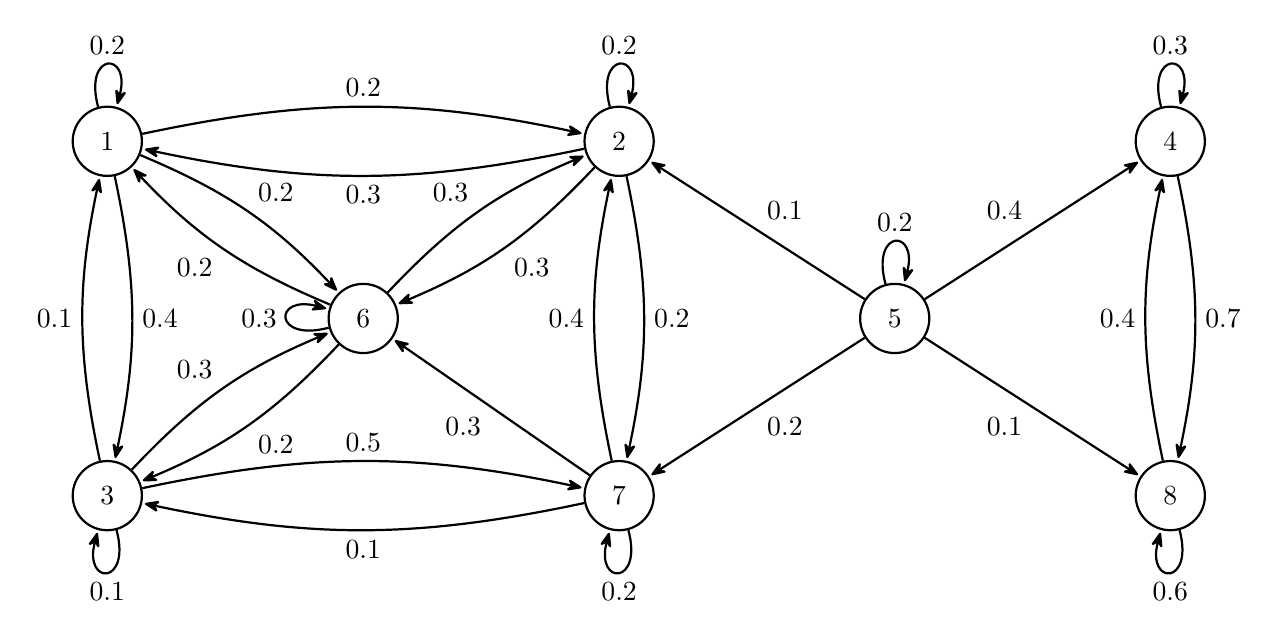
\begin{tikzpicture}[shorten >=1pt,auto,>={Stealth[round]},thick,every node/.style={align=center}]
  \node[state] (s1) at (0,4.5)     {1};
  \node[state] (s2) at (6.5,4.5)   {2};
  \node[state] (s3) at (0,0)       {3};
  \node[state] (s7) at (6.5,0)     {7};
  \node[state] (s6) at (3.25,2.25) {6};
  \node[state] (s5) at (10,2.25)   {5};
  \node[state] (s4) at (13.5,4.5)  {4};
  \node[state] (s8) at (13.5,0)    {8};

  \path[->] (s1) edge [loop above        ] node        {0.2} (s1)
                 edge [bend left = 12    ] node        {0.2} (s2)
                 edge [bend left = 12    ] node        {0.4} (s3)
                 edge [bend left = 12    ] node        {0.2} (s6)
            (s2) edge [loop above        ] node        {0.2} (s2)
                 edge [bend left = 12    ] node        {0.3} (s1)
                 edge [bend left = 12    ] node        {0.3} (s6)
                 edge [bend left = 12    ] node        {0.2} (s7)
            (s3) edge [loop below        ] node        {0.1} (s3)
                 edge [bend left = 12    ] node        {0.1} (s1)
                 edge [bend left = 12    ] node        {0.3} (s6)
                 edge [bend left = 12    ] node        {0.5} (s7)
            (s6) edge [loop left         ] node        {0.3} (s6)
                 edge [bend left = 12    ] node        {0.2} (s1)
                 edge [bend left = 12    ] node        {0.3} (s2)
                 edge [bend left = 12    ] node        {0.2} (s3)
            (s7) edge [loop below        ] node        {0.2} (s7)
                 edge [bend left = 12    ] node        {0.4} (s2)
                 edge [bend left = 12    ] node        {0.1} (s3)
                 edge [                  ] node        {0.3} (s6)
            (s5) edge [loop above        ] node        {0.2} (s5)
                 edge [                  ] node [swap] {0.1} (s2)
                 edge [                  ] node        {0.2} (s7)
                 edge [                  ] node        {0.4} (s4)
                 edge [                  ] node [swap] {0.1} (s8)
            (s4) edge [loop above        ] node        {0.3} (s4)
                 edge [bend left = 12    ] node        {0.7} (s8)
            (s8) edge [loop below        ] node        {0.6} (s8)
                 edge [bend left = 12    ] node        {0.4} (s4);
\end{tikzpicture}
\end{figure}
\subsection*{Решение пункта 1:}
\begin{displaymath}
  \mathbb{P}^{(2)} = \mathbb{P}^2 = \frac{1}{100}
  \begin{pmatrix}
    18 & 14 & 16 & 0 & 0 & 28 & 24 & 0 \\18 & 27 & 20 & 0 & 0 & 27 & 8 & 0 \\9 & 31 & 16 & 0 & 0 & 29 & 15 & 0 \\0 & 0 & 0 & 37 & 0 & 0 & 0 & 63 \\3 & 12 & 2 & 24 & 4 & 9 & 10 & 36 \\21 & 19 & 16 & 0 & 0 & 28 & 16 & 0 \\19 & 25 & 9 & 0 & 0 & 30 & 17 & 0 \\0 & 0 & 0 & 36 & 0 & 0 & 0 & 64
  \end{pmatrix}.
\end{displaymath}

\begin{align*}
  & 18/100 + 14/100 + 16/100 + 0 + 0 + 28/100 + 24/100 + 0 = 1 \text{ - верно} \\
  & 18/100 + 27/100 + 20/100 + 0 + 0 + 27/100 + 8/100 + 0 = 1 \text{ - верно} \\
  & 9/100 + 31/100 + 16/100 + 0 + 0 + 29/100 + 15/100 + 0 = 1 \text{ - верно} \\
  & 0 + 0 + 0 + 37/100 + 0 + 0 + 0 + 63/100 = 1 \text{ - верно} \\
  & 3/100 + 12/100 + 2/100 + 24/100 + 4/100 + 9/100 + 10/100 + 36/100 = 1 \text{ - верно} \\
  & 21/100 + 19/100 + 16/100 + 0 + 0 + 28/100 + 16/100 + 0 = 1 \text{ - верно} \\
  & 19/100 + 25/100 + 9/100 + 0 + 0 + 30/100 + 17/100 + 0 = 1 \text{ - верно} \\
  & 0 + 0 + 0 + 36/100 + 0 + 0 + 0 + 64/100 = 1 \text{ - верно}
\end{align*}
\subsection*{Решение пункта 2:}
Цепь состоит из 3 классов сообщающихся состояний:
\(\mathbf{C}_1 = \{1, 2, 3, 6, 7\}\), \(\mathbf{C}_2 = \{4, 8\}\) и \(\mathbf{C}_3 = \{5\}\).

\begin{table}[H]
\centering
\begin{minipage}[t]{.72\textwidth}
\begin{center}
\begin{tabular}[t]{c|ccccc}
\(\mathbf{C}_1\) & 1 & 2 & 3 & 6 & 7\\
\hline
1 & 1 \(\to\) 1 & 1 \(\to\) 2 & 1 \(\to\) 3 & 1 \(\to\) 6 & 1 \(\to\) 2 \(\to\) 7\\
2 & 2 \(\to\) 1 & 2 \(\to\) 2 & 2 \(\to\) 1 \(\to\) 3 & 2 \(\to\) 6 & 2 \(\to\) 7\\
3 & 3 \(\to\) 1 & 3 \(\to\) 6 \(\to\) 2 & 3 \(\to\) 3 & 3 \(\to\) 6 & 3 \(\to\) 7\\
6 & 6 \(\to\) 1 & 6 \(\to\) 2 & 6 \(\to\) 3 & 6 \(\to\) 6 & 6 \(\to\) 2 \(\to\) 7\\
7 & 7 \(\to\) 2 \(\to\) 1 & 7 \(\to\) 2 & 7 \(\to\) 3 & 7 \(\to\) 6 & 7 \(\to\) 7\\
\end{tabular}
\end{center}
\end{minipage}
\begin{minipage}[t]{.26\textwidth}
\begin{center}
\begin{tabular}[t]{c|cc}
\(\mathbf{C}_2\) & 4 & 8\\
\hline
4 & 4 \(\to\) 4 & 4 \(\to\) 8\\
8 & 8 \(\to\) 4 & 8 \(\to\) 8\\
\end{tabular}
\end{center}
\end{minipage}
\end{table}

Состояние 5 - класс \(\mathbf{C}_3 = \{5\}\), сообщается само с собой
(\(5 \to 5\), \(p_{55} = 0.2\)), только он незамкнутый (из 5 есть переходы в 2, 4, 7, 8).

Вершина 5 - недостижимая из любой другой вершины (т.к. \(\exists\) пути
из нее, но в нее нет) \(\Rightarrow\) вершина 5 несущественная.

\subsection*{Решение пункта 3:}
Так как несущественные состояния - невозвратные, то вершина 5 невозвратная.

\subsection*{Решение пункта 4:}
Период класса \(T = \text{НОД}(T_n)\), где \(T_n = \{n \geq 1 : p^{(n)}_{ii} > 0\}\) -
длины всех возвратов в состояние \(i\) класса. У каждого состояния есть петля
(\(p_{ii} > 0\)), поэтому \(p^{(n)}_{ii} \geq (p_{ii})^n > 0\) при любом \(n\):

\begin{displaymath}
  \mathbf{C}_1 = \{1, 2, 3, 6, 7\},\ \mathbf{C}_2 = \{4, 8\},\ \mathbf{C}_3 = \{5\}: \quad
  T_n = \{1, 2, 3, \ldots\}, \quad T = \text{НОД}(1, 2, 3, \ldots) = 1
\end{displaymath}

Все классы непериодичны.

\subsection*{Решение пункта 5:}
Вектор финальных вероятностей класса \(\mathbf{C}_i\):
\(\pi_{\mathbf{C}_i} =
\pi_{\mathbf{C}_i}\cdot\mathbb{P}_{\mathbf{C}_i}\).

\begin{displaymath}
  \pi_{\mathbf{C}_1} = \left(\pi_1, \pi_2, \pi_3, \pi_6, \pi_7\right),\qquad
  \mathbb{P}_{\mathbf{C}_1} = \frac{1}{10}
  \begin{pmatrix}
    2 & 2 & 4 & 2 & 0 \\
    3 & 2 & 0 & 3 & 2 \\
    1 & 0 & 1 & 3 & 5 \\
    2 & 3 & 2 & 3 & 0 \\
    0 & 4 & 1 & 3 & 2 \\
  \end{pmatrix}
\end{displaymath}
\begin{displaymath}
  \left\{\begin{aligned}
    & 10\pi_1 = 2\pi_1 + 3\pi_2 +  \pi_3 + 2\pi_6 \\
    & 10\pi_2 = 2\pi_1 + 2\pi_2 + 3\pi_6 + 4\pi_7 \\
    & 10\pi_3 = 4\pi_1 +  \pi_3 + 2\pi_6 +  \pi_7 \\
    & 10\pi_6 = 2\pi_1 + 3\pi_2 + 3\pi_3 + 3\pi_6 + 3\pi_7 \\
    & 10\pi_7 = 2\pi_2 + 5\pi_3 + 2\pi_7 \\
    &  1    =  \pi_1 +  \pi_2 +  \pi_3 +  \pi_6 +  \pi_7 \\
  \end{aligned}\right.\Rightarrow
  \left\{\begin{aligned}
    & \pi_1 = \frac{1769}{10063} \approx 0.1758 \\
    & \pi_2 = \frac{2292}{10063} \approx 0.2278 \\
    & \pi_3 = \frac{1592}{10063} \approx 0.1582 \\
    & \pi_6 = \frac{2842}{10063} \approx 0.2824 \\
    & \pi_7 = \frac{1568}{10063} \approx 0.1558 \\
  \end{aligned}\right.
\end{displaymath}

\begin{displaymath}
  \pi_{\mathbf{C}_2} = \left(\pi_4, \pi_8\right),\qquad
  \mathbb{P}_{\mathbf{C}_2} = \frac{1}{10}
  \begin{pmatrix}
    3 & 7 \\
    4 & 6 \\
  \end{pmatrix}
\end{displaymath}
\begin{displaymath}
  \left\{\begin{aligned}
    & 10\pi_4 = 3\pi_4 + 4\pi_8 \\
    & 10\pi_8 = 7\pi_4 + 6\pi_8 \\
    &  1    =  \pi_4 +  \pi_8 \\
  \end{aligned}\right.\Rightarrow
  \left\{\begin{aligned}
    & \pi_4 = \frac{4}{11} \approx 0.3636 \\
    & \pi_8 = \frac{7}{11} \approx 0.6364 \\
  \end{aligned}\right.
\end{displaymath}

Для незамкнутого класса \(\mathbf{C}_3 = \{5\}\): \(\pi_5 = 0\), так как состояние 5 невозвратное.
\subsection*{Решение пункта 6:}
Поиск траектории был реализован на языке python. 
Для разных классов сообщающихся состояний для различных вершин были рассмотрены траектории длины
10, 50, 100, 1000.

Функция simulate\_markov\_chain моделирует траекторию цепи - на каждом шаге
следующее состояние выбирается случайно с вероятностями из строки матрицы переходов
для текущего состояния.
\begin{lstlisting}[caption={Функция моделирования траектории цепи Маркова}]
def simulate_markov_chain(transition_matrix, initial_state, steps):
    states = [initial_state]
    current_state = initial_state

    for _ in range(steps):
        current_state = np.random.choice(
            a=len(transition_matrix),
            p=transition_matrix[current_state]
        )
        states.append(current_state)

    return states
\end{lstlisting}

Результаты (Initial State - начальное состояние, Steps - число шагов,
Trajectory - полученная траектория, то есть последовательность состояний цепи):

{\small\setstretch{1}
Initial State: 1, Steps: 10, Trajectory: [1, 2, 6, 3, 1, 2, 1, 3, 3, 1, 6]

Initial State: 5, Steps: 50, Trajectory: [5, 5, 2, 6, 1, 2, 1, 3, 6, 2, 2, 1, 6, 3, 6, 2, 1, 3, 7, 6, 6, 1, 3, 1, 3, 6, 2, 6, 3, 6, 1, 3, 7, 2, 6, 2, 1, 1, 2, 7, 2, 2, 1, 3, 6, 6, 3, 6, 6, 6, 6]

Initial State: 3, Steps: 100, Trajectory: [3, 6, 6, 1, 3, 7, 6, 3, 7, 6, 6, 1, 1, 3, 6, 2, 1, 1, 3, 7, 6, 6, 6, 2, 2, 1, 6, 6, 6, 1, 3, 7, 2, 7, 2, 6, 1, 6, 3, 7, 7, 3, 7, 6, 2, 1, 3, 7, 7, 6, 1, 2, 6, 1, 2, 1, 6, 6, 2, 2, 6, 3, 7, 6, 3, 3, 7, 2, 1, 6, 3, 7, 6, 6, 3, 3, 7, 2, 7, 2, 7, 2, 6, 1, 1, 3, 7, 2, 6, 2, 1, 3, 1, 6, 1, 6, 6, 1, 3, 7, 2]

Initial State: 6, Steps: 1000, Trajectory: [6, 3, 7, 2, 1, 3, 7, 7, 6, 2, 1, 2, 6, 6, 6, 1, 3, 6, 3, 1, 3, 7, 2, 2, 1, 3, 1, 2, 6, 6, 1, 1, 2, 6, 1, 3, 6, 6, 6, 6, 2, 2, 7, 6, 6, 3, 6, 6, 3, 7, 2, 1, 2, 6, 3, 6, 6, 1, 2, 1, 2, 7, 6, 1, 1, 1, 1, 1, 2, 6, 6, 1, 3, 7, 2, 6, 3, 7, 7, 2, 6, 1, 1, 2, 6, 1, 2, 6, 1, 6, 6, 6, 6, 6, 3, 3, 7, 2, 7, 7, 6, 1, 2, 2, 7, 7, 3, 7, 2, 1, 3, 6, 1, 1, 1, 2, 6, 6, 6, 2, 1, 1, 1, 3, 6, 3, 1, 3, 6, 1, 6, 6, 1, 2, 1, 6, 6, 3, 7, 3, 3, 6, 6, 1, 3, 6, 1, 3, 3, 1, 2, 1, 3, 7, 2, 1, 1, 3, 1, 2, 7, 7, 6, 6, 6, 2, 6, 2, 7, 7, 7, 2, 2, 2, 1, 6, 1, 2, 1, 2, 1, 2, 7, 6, 2, 6, 6, 6, 6, 3, 6, 2, 6, 3, 7, 2, 7, 6, 2, 1, 3, 6, 2, 7, 7, 3, 7, 6, 2, 1, 3, 3, 7, 2, 2, 2, 7, 6, 2, 1, 6, 2, 6, 1, 2, 2, 7, 6, 6, 1, 3, 6, 3, 6, 2, 6, 1, 3, 7, 6, 1, 3, 6, 3, 6, 6, 3, 6, 2, 2, 1, 1, 2, 1, 2, 2, 6, 2, 2, 6, 6, 2, 7, 2, 1, 3, 6, 1, 1, 3, 6, 2, 7, 6, 2, 1, 2, 6, 3, 7, 7, 7, 7, 3, 6, 6, 2, 7, 2, 2, 6, 6, 1, 2, 7, 2, 6, 6, 6, 2, 2, 1, 6, 2, 1, 3, 7, 2, 1, 6, 6, 2, 1, 2, 7, 3, 7, 6, 3, 6, 1, 1, 3, 6, 1, 3, 7, 2, 7, 2, 7, 2, 6, 1, 3, 6, 6, 6, 6, 6, 2, 7, 2, 1, 2, 7, 7, 2, 6, 1, 2, 1, 2, 2, 6, 6, 6, 6, 6, 3, 6, 6, 3, 6, 6, 2, 1, 1, 3, 7, 2, 6, 1, 3, 6, 3, 3, 6, 2, 1, 6, 2, 1, 3, 6, 6, 1, 6, 1, 1, 3, 7, 3, 3, 7, 2, 2, 1, 3, 3, 1, 2, 6, 6, 2, 7, 6, 2, 7, 6, 6, 6, 2, 6, 2, 1, 3, 3, 7, 6, 1, 2, 6, 3, 7, 7, 7, 2, 7, 7, 6, 3, 7, 7, 2, 1, 6, 2, 6, 6, 6, 3, 1, 1, 3, 6, 6, 3, 3, 7, 2, 1, 3, 3, 7, 2, 1, 2, 2, 7, 2, 2, 7, 3, 7, 7, 2, 1, 3, 3, 6, 1, 2, 1, 3, 7, 2, 1, 3, 7, 2, 1, 2, 2, 1, 6, 6, 6, 2, 1, 3, 1, 2, 2, 2, 6, 1, 6, 1, 3, 1, 6, 2, 2, 7, 7, 2, 2, 1, 3, 3, 3, 7, 6, 1, 3, 7, 2, 1, 2, 6, 2, 7, 3, 7, 2, 6, 6, 2, 1, 3, 6, 6, 2, 6, 3, 7, 2, 2, 6, 3, 6, 3, 7, 6, 2, 2, 7, 6, 6, 2, 7, 7, 2, 6, 3, 7, 3, 7, 2, 6, 6, 6, 2, 1, 3, 6, 1, 3, 1, 3, 7, 6, 6, 2, 1, 3, 6, 1, 6, 3, 3, 3, 6, 6, 3, 6, 3, 7, 6, 2, 6, 6, 6, 2, 2, 6, 2, 7, 7, 6, 2, 6, 2, 7, 6, 2, 6, 1, 3, 7, 2, 1, 2, 2, 2, 2, 2, 1, 6, 6, 1, 6, 6, 6, 2, 1, 6, 2, 1, 1, 3, 6, 1, 3, 1, 3, 7, 6, 2, 1, 3, 6, 1, 1, 2, 7, 2, 2, 1, 2, 2, 1, 1, 3, 3, 7, 6, 6, 2, 2, 6, 2, 7, 6, 3, 7, 2, 6, 6, 1, 1, 3, 1, 2, 6, 2, 2, 7, 2, 7, 2, 2, 7, 2, 7, 7, 7, 6, 1, 3, 7, 7, 6, 3, 7, 6, 3, 1, 1, 1, 6, 6, 3, 6, 3, 7, 2, 1, 3, 7, 6, 6, 2, 7, 7, 7, 2, 1, 2, 1, 3, 7, 6, 2, 7, 2, 2, 7, 6, 2, 1, 3, 7, 2, 7, 2, 7, 2, 1, 1, 3, 7, 2, 6, 6, 6, 2, 1, 1, 1, 2, 2, 7, 6, 2, 7, 2, 2, 2, 7, 6, 6, 6, 1, 6, 1, 3, 7, 2, 6, 6, 3, 7, 2, 7, 6, 6, 3, 3, 6, 6, 1, 6, 6, 2, 7, 6, 2, 1, 1, 3, 6, 6, 2, 7, 6, 1, 2, 7, 6, 3, 7, 6, 3, 7, 2, 1, 2, 6, 1, 6, 6, 2, 6, 6, 6, 1, 2, 6, 2, 1, 3, 6, 1, 2, 6, 2, 6, 2, 7, 2, 1, 3, 6, 2, 1, 3, 6, 3, 7, 3, 6, 6, 6, 3, 6, 2, 1, 3, 3, 1, 2, 7, 2, 6, 3, 6, 2, 1, 1, 6, 1, 1, 6, 2, 6, 6, 3, 7, 2, 2, 6, 2, 2, 6, 2, 1, 3, 7, 7, 2, 2, 6, 6, 2, 1, 3, 7, 2, 1, 6, 2, 1, 3, 6, 3, 3, 7, 7, 6, 2, 1, 1, 6, 6, 6, 3, 6, 6, 2, 1, 2, 6, 2, 1, 1, 1, 2, 6, 2, 7, 2, 2, 7, 2, 1, 3, 7, 2, 7, 6, 2, 2, 2, 7, 6, 6, 6, 2, 1, 3, 7, 2, 7, 2, 7, 3, 7, 7, 7, 6, 2, 6, 1, 2, 6, 6, 1, 1, 3, 6, 1, 3, 3, 7, 7, 6, 6, 3, 1, 2, 2, 2, 6, 3, 3, 6, 2, 2, 2, 2, 6, 3, 7, 7, 3, 6, 2, 6, 1, 3, 1, 2, 2, 6, 1, 6, 2, 1, 1]

Initial State: 4, Steps: 100, Trajectory: [4, 8, 4, 4, 8, 4, 4, 8, 8, 8, 4, 8, 8, 4, 8, 8, 8, 8, 4, 8, 8, 8, 8, 8, 8, 8, 8, 4, 4, 8, 8, 8, 8, 8, 4, 8, 8, 8, 8, 8, 8, 4, 4, 4, 8, 8, 8, 4, 8, 8, 4, 8, 4, 8, 8, 8, 8, 8, 8, 4, 4, 8, 4, 8, 8, 4, 8, 8, 4, 8, 4, 8, 4, 8, 4, 8, 8, 4, 8, 8, 4, 8, 8, 4, 8, 8, 4, 8, 8, 8, 8, 8, 8, 4, 4, 8, 8, 8, 4, 8, 8]

Initial State: 8, Steps: 1000, Trajectory: [8, 8, 4, 4, 8, 8, 8, 8, 8, 8, 8, 8, 8, 8, 8, 8, 8, 4, 4, 8, 8, 8, 8, 8, 4, 4, 8, 8, 8, 4, 8, 4, 8, 4, 8, 4, 4, 8, 4, 4, 4, 4, 4, 8, 4, 8, 8, 8, 8, 8, 4, 8, 8, 8, 8, 4, 4, 4, 4, 8, 8, 8, 8, 4, 8, 8, 4, 4, 8, 8, 8, 8, 8, 8, 8, 4, 4, 8, 8, 8, 4, 4, 4, 8, 4, 8, 4, 8, 8, 8, 4, 4, 8, 4, 8, 4, 8, 8, 8, 4, 8, 8, 8, 4, 8, 8, 4, 8, 4, 8, 4, 4, 4, 8, 8, 4, 4, 4, 8, 8, 4, 8, 4, 4, 4, 8, 8, 8, 8, 8, 8, 4, 8, 8, 4, 8, 4, 8, 8, 8, 4, 4, 8, 8, 8, 4, 4, 8, 8, 4, 8, 8, 8, 4, 8, 8, 8, 4, 8, 8, 4, 8, 4, 8, 8, 4, 4, 8, 8, 4, 8, 4, 8, 8, 8, 4, 8, 4, 4, 8, 4, 8, 8, 4, 8, 4, 4, 8, 4, 8, 4, 8, 8, 8, 8, 8, 8, 8, 8, 8, 4, 8, 4, 8, 4, 8, 8, 4, 8, 8, 4, 8, 4, 8, 4, 8, 4, 8, 8, 8, 4, 8, 8, 8, 8, 4, 8, 4, 8, 8, 8, 8, 8, 4, 8, 8, 4, 8, 8, 8, 8, 8, 4, 8, 8, 8, 8, 4, 8, 4, 8, 8, 8, 8, 4, 8, 8, 8, 4, 4, 4, 4, 8, 8, 4, 8, 8, 8, 4, 8, 8, 8, 8, 4, 4, 8, 8, 4, 8, 8, 4, 8, 4, 8, 8, 4, 8, 8, 8, 8, 8, 8, 8, 8, 8, 8, 4, 4, 4, 4, 8, 8, 4, 8, 4, 8, 8, 8, 4, 4, 8, 4, 8, 8, 8, 4, 4, 8, 8, 8, 8, 4, 8, 4, 8, 8, 8, 4, 8, 4, 8, 8, 8, 8, 4, 8, 8, 8, 4, 8, 8, 8, 8, 8, 4, 8, 8, 8, 8, 8, 4, 4, 8, 4, 8, 8, 8, 8, 8, 8, 8, 8, 8, 8, 8, 4, 8, 4, 8, 4, 4, 8, 8, 4, 8, 8, 8, 8, 8, 4, 8, 4, 8, 8, 4, 4, 8, 8, 4, 8, 4, 8, 8, 8, 8, 8, 8, 8, 4, 8, 4, 4, 4, 8, 8, 8, 8, 4, 8, 8, 4, 8, 8, 8, 8, 8, 4, 4, 4, 8, 8, 4, 8, 8, 8, 4, 8, 8, 8, 4, 8, 8, 8, 4, 8, 8, 8, 4, 8, 8, 8, 4, 8, 8, 8, 8, 8, 8, 4, 4, 8, 8, 8, 4, 4, 4, 8, 8, 4, 8, 4, 4, 8, 4, 8, 8, 4, 8, 8, 8, 4, 8, 8, 4, 8, 8, 4, 8, 4, 4, 8, 8, 8, 4, 8, 8, 8, 8, 8, 4, 8, 4, 8, 8, 8, 4, 8, 8, 4, 4, 8, 8, 4, 8, 8, 8, 8, 4, 4, 8, 8, 4, 4, 4, 8, 4, 8, 8, 8, 4, 8, 8, 4, 4, 8, 8, 8, 8, 8, 8, 8, 8, 8, 4, 8, 8, 4, 4, 8, 4, 8, 8, 8, 4, 4, 8, 8, 8, 4, 8, 8, 4, 4, 8, 8, 8, 4, 8, 8, 8, 8, 4, 8, 8, 4, 8, 4, 4, 8, 8, 8, 8, 4, 8, 4, 4, 8, 8, 8, 8, 4, 8, 4, 8, 4, 4, 8, 4, 8, 4, 4, 8, 8, 8, 8, 8, 8, 8, 8, 8, 8, 8, 8, 8, 8, 8, 4, 8, 8, 8, 8, 8, 8, 4, 8, 8, 8, 4, 8, 4, 8, 8, 4, 8, 8, 4, 4, 8, 8, 8, 8, 4, 8, 8, 8, 8, 4, 8, 8, 4, 8, 8, 8, 4, 8, 4, 4, 4, 8, 8, 4, 8, 8, 8, 4, 4, 8, 8, 8, 8, 8, 4, 4, 8, 4, 8, 4, 4, 8, 8, 8, 8, 4, 4, 8, 4, 8, 4, 4, 4, 4, 4, 8, 8, 8, 4, 4, 8, 4, 4, 8, 8, 8, 8, 8, 8, 8, 8, 8, 8, 4, 8, 8, 8, 8, 4, 8, 8, 4, 4, 8, 8, 8, 8, 8, 4, 8, 8, 8, 8, 8, 4, 4, 8, 4, 8, 4, 4, 8, 8, 4, 8, 4, 8, 8, 4, 4, 8, 4, 8, 4, 8, 4, 4, 8, 4, 8, 8, 4, 4, 4, 8, 8, 8, 8, 8, 8, 8, 8, 4, 8, 4, 8, 8, 8, 8, 8, 8, 4, 4, 8, 8, 8, 8, 4, 4, 4, 8, 4, 4, 8, 8, 8, 4, 4, 8, 8, 4, 8, 8, 8, 8, 4, 8, 8, 8, 4, 8, 8, 8, 8, 8, 8, 8, 4, 4, 4, 8, 8, 8, 8, 8, 8, 8, 8, 8, 4, 8, 8, 8, 4, 8, 8, 8, 8, 4, 8, 8, 8, 8, 4, 4, 8, 8, 4, 8, 4, 8, 8, 4, 4, 8, 8, 8, 4, 8, 4, 8, 4, 4, 4, 8, 8, 8, 8, 4, 4, 4, 8, 8, 8, 8, 4, 4, 4, 8, 8, 4, 4, 8, 8, 4, 4, 8, 8, 8, 4, 8, 4, 8, 8, 8, 8, 4, 8, 4, 4, 4, 8, 8, 8, 8, 8, 4, 8, 4, 8, 8, 4, 8, 8, 8, 8, 8, 8, 8, 8, 4, 8, 4, 8, 8, 8, 8, 8, 8, 8, 8, 8, 4, 8, 8, 4, 8, 8, 8, 8, 4, 4, 8, 8, 8, 8, 8, 8, 8, 8, 8, 8, 8, 8, 8, 8, 8, 8, 4, 8, 4, 8, 4, 8, 4, 8, 8, 8, 4, 8, 8, 8, 8, 4, 8, 8, 4, 4, 8, 8, 8, 4, 4, 8, 8, 8, 8, 8, 4, 8, 4, 8, 4, 8, 4, 8, 8, 4, 8, 4, 4, 8, 4, 8, 8, 8, 4, 8, 8, 8, 4, 8, 8, 8]
\par}

По траекториям видно что не происходит выхода из класса сообщающихся
состояний. Из несущественного состояния 5 цепь уходит в класс \(\mathbf{C}_1\) и
больше в 5 не возвращается.

\subsection*{Решение пункта 7:}
Граф марковской цепи был разбит на классы (пункт 2), рассматриваются замкнутые классы
\(\mathbf{C}_1 = \{1, 2, 3, 6, 7\}\) и \(\mathbf{C}_2 = \{4, 8\}\). Так как классы
непериодичны то для них были взяты матрицы переходов \(\mathbb{P}_{\mathbf{C}_1}\) и
\(\mathbb{P}_{\mathbf{C}_2}\) из пункта 5. Траектории внутри класса моделируются
функцией simulate\_markov\_chain из пункта 6.

Функция calculate\_state\_percentages считает долю времени, проведенного
цепью в каждом состоянии: число попаданий в состояние, деленное на длину траектории.
\begin{lstlisting}[caption={Функция подсчета доли времени в каждом состоянии}]
def calculate_state_percentages(states, num_states):
    counts = np.bincount(states, minlength=num_states)
    percentages = counts / len(states)
    return percentages
\end{lstlisting}

Функция stationary\_distribution находит вектор финальных вероятностей как
собственный вектор матрицы \(\mathbb{P}^T\) для собственного значения 1, нормированный
так, чтобы сумма была равна 1.
\begin{lstlisting}[caption={Функция нахождения вектора финальных вероятностей}]
def stationary_distribution(transition_matrix):
    eigenvalues, eigenvectors = np.linalg.eig(transition_matrix.T)
    stationary_vector = eigenvectors[:, np.isclose(eigenvalues, 1)]
    stationary_vector = stationary_vector / np.sum(stationary_vector)
    return stationary_vector.real.flatten()
\end{lstlisting}

Функция simulation моделирует траекторию заданной длины из заданного
состояния и печатает доли времени, вектор финальных вероятностей и модуль их разности.
\begin{lstlisting}[caption={Функция моделирования и сравнения с финальными вероятностями}]
def simulation(steps, initial_state, transition_matrix, labels):
    print(f"Initial state: {labels[initial_state]}, steps: {steps}")

    trajectory = simulate_markov_chain(transition_matrix, initial_state, steps)

    percentages = calculate_state_percentages(trajectory, len(transition_matrix))
    print(f"Percentages: {percentages}")
    stationary_vector = stationary_distribution(transition_matrix)
    print(f"Final distribution: {stationary_vector}")

    difference = np.abs(percentages - stationary_vector)
    print(f"Difference: {difference}\n")
\end{lstlisting}

Результаты (Initial state - начальное состояние, steps - число шагов,
Percentages - доля времени в каждом состоянии класса, Final distribution - вектор
финальных вероятностей класса, Difference - модуль разности этих векторов):

{\setstretch{1}\small
\begin{verbatim}
Class 1: states (1, 2, 3, 6, 7)

Initial state: 1, steps: 10
Percentages: [0.3636 0.1818 0.2727 0.1818 0.    ]
Final distribution: [0.1758 0.2278 0.1582 0.2824 0.1558]
Difference: [0.1878 0.0459 0.1145 0.1006 0.1558]

Initial state: 2, steps: 50
Percentages: [0.1765 0.2157 0.2157 0.3137 0.0784]
Final distribution: [0.1758 0.2278 0.1582 0.2824 0.1558]
Difference: [0.0007 0.0121 0.0575 0.0313 0.0774]

Initial state: 3, steps: 100
Percentages: [0.1881 0.1683 0.1782 0.2871 0.1782]
Final distribution: [0.1758 0.2278 0.1582 0.2824 0.1558]
Difference: [0.0123 0.0594 0.02   0.0047 0.0224]

Initial state: 6, steps: 1000
Percentages: [0.1798 0.2438 0.1508 0.2747 0.1508]
Final distribution: [0.1758 0.2278 0.1582 0.2824 0.1558]
Difference: [0.004  0.016  0.0074 0.0077 0.005 ]

Class 2: states (4, 8)

Initial state: 4, steps: 10
Percentages: [0.5455 0.4545]
Final distribution: [0.3636 0.6364]
Difference: [0.1818 0.1818]

Initial state: 8, steps: 50
Percentages: [0.2549 0.7451]
Final distribution: [0.3636 0.6364]
Difference: [0.1087 0.1087]

Initial state: 4, steps: 100
Percentages: [0.3564 0.6436]
Final distribution: [0.3636 0.6364]
Difference: [0.0072 0.0072]

Initial state: 8, steps: 1000
Percentages: [0.3407 0.6593]
Final distribution: [0.3636 0.6364]
Difference: [0.023 0.023]
\end{verbatim}
}

Получается чем длиннее траектория - тем ближе вектор процентов
времени нахождения к вектору финальных вероятностей (в классе 2 при
N = 1000 отклонение 0.023, а при N = 100 отклонение вышло меньше: 0.0072).

Вектора финальных вероятностей
совпали с посчитанными в пункте 5.
\end{document}
